\documentclass[11pt]{article}

%%%%%%%%%%%%%%%%%%%%%%%%%%%%%%%%%%%%%%%%%%%%%%%%%%%%%%%%%%%%%%%%%%%%
%%%%%%%%%%%%%%%%%%%%%%%%%%   Package     %%%%%%%%%%%%%%%%%%%%%%%%%%%
%%%%%%%%%%%%%%%%%%%%%%%%%%%%%%%%%%%%%%%%%%%%%%%%%%%%%%%%%%%%%%%%%%%%

\usepackage{amsmath, amssymb, amsthm, mathtools, empheq, dsfont}
\usepackage{graphicx}
\usepackage{array}
\usepackage[colorlinks=true, allcolors=blue]{hyperref}
\usepackage{fullpage}
\usepackage[english]{babel}
\usepackage{subcaption}
\captionsetup[subfigure]{justification=centering}
\usepackage{titlesec}
\usepackage{changepage}
\usepackage{tikz}
\usepackage{setspace}
\usepackage{titlesec}
\usepackage{lmodern}

\usepackage[font=scriptsize, labelfont=bf]{caption}
\usepackage{geometry}
\geometry{hmargin=2.5cm,vmargin=2.5cm}

\renewcommand{\thesection}{\Roman{section}}

%%%%%%%%%%%%%%%%%%%%%%%%%%%%%%%%%%%%%%%%%%%%%%%%%%%%%%%%%%%%%%%%%%%%
%%%%%%%%%%%%%%%%%%%%%%%   Math commands     %%%%%%%%%%%%%%%%%%%%%%%%
%%%%%%%%%%%%%%%%%%%%%%%%%%%%%%%%%%%%%%%%%%%%%%%%%%%%%%%%%%%%%%%%%%%%

\newcommand{\HRule}{\rule{\linewidth}{0.5mm}} %Pour la page de garde
\newcommand\numberthis{\addtocounter{equation}{1}\tag{\theequation}}

\newcommand{\hamiltonian}{\hat{H}}
\newcommand{\transition}{\hat{T}}
\newcommand{\transmatrix}[1]{M_{{#1}}^\qvector}

\newcommand{\position}{\mathbf{\hat{r}}}
\newcommand{\impulsion}{\mathbf{\hat{p}}}
\newcommand{\kvector}{\mathbf{k}}
\newcommand{\qvector}{\mathbf{q}}
\newcommand{\rvector}{\mathbf{r}}

\newcommand{\polarization}{\boldsymbol{\mathbf{\epsilon}}}

\newcommand{\spin}{\mathbf{\hat{S}}}
\newcommand{\magneticfield}{\mathbf{B}}
\newcommand{\vectorpotential}{\mathbf{\hat{A}}}

\newcommand{\pcreation}[1]{\hat{a}_{{#1}}^{\dagger}}
\newcommand{\pannihilation}[1]{\hat{a}_{{#1}}^{\phantom{\dagger}}}
\newcommand{\creation}[1]{\hat{c}_{{#1}}^{\dagger}}
\newcommand{\annihilation}[1]{\hat{c}_{{#1}}^{\phantom{\dagger}}}
\newcommand{\occupation}[1]{\hat{n}_{{#1}}}

\newcommand{\ket}[1]{\left| {#1} \right>}
\newcommand{\bra}[1]{\left< {#1} \right|}
\newcommand{\braket}[2]{\left< {#1} | {#2} \right>}

\newcommand{\angstrom}{\mathring{A}}

\newcommand{\bath}{\text{bath}}
\newcommand{\imp}{\text{imp}}
\newcommand{\empti}{\text{empty}}
\newcommand{\filled}{\text{filled}}
\newcommand{\activ}{\text{active}}
\newcommand{\dxy}{d_{x^2-y^2}}

%%%%%%%%%%%%%%%%%%%%%%%%%%%%%%%%%%%%%%%%%%%%%%%%%%%%%%%%%%%%%%%%%%%%
%%%%%%%%%%%%%%%%%%%%%%%   Page de garde     %%%%%%%%%%%%%%%%%%%%%%%%
%%%%%%%%%%%%%%%%%%%%%%%%%%%%%%%%%%%%%%%%%%%%%%%%%%%%%%%%%%%%%%%%%%%%


% Titre et auteur
\title{\LARGE \textbf{Natural Orbitals : Theory and Applications}}
\author{\large M. \textsc{Vinteler}, C. \textsc{Letouzé}, S. \textsc{Paeckel}, B. \textsc{Lenz}, G. \textsc{Radtke}}
\date{August 2026}
\makeatletter

\begin{document}
\begin{center}
    \@title \\
    \vspace{0.1cm}
    \@author
\end{center}
{\color{blue}[MV : Maxime comment]}\\
{\color{violet}[CL : Coraline comment]}\\
{\color{teal}[SB : Sebastian comment]}\\
{\color{red}[BL : Benjamin comment]}\\
{\color{orange}[GR : Guillaume comment]}
\section{Theory on Natural Orbitals}\label{section:intro}
This part of the notes is mainly inspired from \cite{kaye_natural_nodate, lu_natural-orbital_2019, lu_efficient_2014}.\\
Natural orbitals correspond to a change of basis of the naïve star representation of the Anderson impurity model (AIM). This transformation allows us to separate the bath into two parts: an active part and an inactive part, the latter being considered as a single Slater determinant and therefore becoming trivial for subsequent calculations (DMRG, ED, ...). Natural orbitals thus reduce the number of degrees of freedom to those associated with the active bath sites. In the MPS framework, this reduction can significantly reduce the required bond dimension.\\
Let us consider a one-band, spin-independent AIM (see also Fig. \ref{subfig:star_rep}):
\begin{equation}\label{eq:star_rep}
\hamiltonian_\star = U \occupation{0\uparrow}\occupation{0\downarrow} + \epsilon_0 (\occupation{0\uparrow} + \occupation{0\downarrow}) + \sum_{l=1,\sigma}^{N_{\text{bath}}} \epsilon_l \occupation{l\sigma} + V_l(\creation{0\sigma} \annihilation{l\sigma} + h.c.) = U \occupation{0\uparrow}\occupation{0\downarrow} + \hamiltonian_\star^{1B}
\end{equation}
where site $0$ corresponds to the impurity and $\hamiltonian_\star^{1B}$ the one-body part of the AIM. We assume that we have access to the correlation matrix $C_{ij\sigma}$ (or density matrix) of the ground state $\ket{\psi_{GS}}$ of the AIM, calculated using DMRG:
\begin{equation}\label{eq:dm}
C_{ij} = \bra{\psi_{GS}}\creation{i}\annihilation{j}\ket{\psi_{GS}}
\end{equation}
where we omit the spin index. The correlation matrix can also be written in terms of its impurity and bath components:
\begin{equation}
C =
\begin{pmatrix}
\rho_{\imp} & \rho_{ib} \\
\rho_{bi} & \rho_{\bath}
\end{pmatrix}
\end{equation}
The next step consists of diagonalizing the bath part of the density matrix, $\rho_{\bath}$. We do not diagonalize the full correlation matrix in order to avoid mixing the impurity site with the bath sites and therefore losing the locality of the impurity.\\
Because of the local interaction on the impurity, the new occupations are not strictly equal to $0$ or $1$. However, most of them remain very close to these values and can therefore be considered as part of a single Slater determinant below a threshold $\epsilon$, a tunable parameter controlling the trade-off between accuracy and computation cost. Furthermore, from the properties of Gaussian states, there exists a single eigenvalue equal to $1-\nu_0$, with $\nu_0=\nu_\imp=C_{00}$ being the impurity occupation {\color{blue}{[MV: still true for interacting calculations ?]}}, which is called the \textit{active site} $\ket{b}$. In ascending order,
\begin{equation}
P^\dagger_\bath \rho_\bath P_\bath =
\text{diag}(\nu_1, \nu_2, \ldots, \nu_{N_\empti}, \ldots, \nu_\activ, \ldots, \nu_{N_\filled}, \ldots, \nu_{N_\bath})
\end{equation}
where we define the inactive empty bath part $\mathcal{E}_I$ as $i\in \{1,\ldots, N_\empti\}$, for which $\nu_i < \epsilon$, and the inactive filled bath part $\mathcal{F}_I$ as $j\in \{N_\filled,\ldots, N_\bath\}$, for which $\nu_j > 1-\epsilon$. The active part $\mathcal{A}$ is defined by $k\in \{N_\empti+1,\ldots, N_\filled-1\}$. The first two spaces will eventually be treated as single Slater determinants, once they are fully decoupled from the active and impurity sites at the end of the natural orbital transformation.\\
For now, we consider the (almost) empty space $\mathcal{E}$ as $m\in \{1,\ldots, N_\activ-1\}$ and the (almost) filled space $\mathcal{F}$ as $n\in \{N_\activ+1,\ldots, N_\bath\}$. Applying this change of basis gives (Fig. \ref{subfig:h_prime_rep})
\begin{equation}\label{eq:bath_rotation}
\hamiltonian' = P^\dagger\hamiltonian_\star^{1B} P, \quad P =
\begin{pmatrix}
1 & 0 \\
0 & P_\bath
\end{pmatrix}
\end{equation}
After this transformation, the impurity and active states are still strongly hybridized with the empty and filled states. However, the hopping between the empty $\mathcal{E}$ states and the filled $\mathcal{F}$ states is now almost zero (Fig. \ref{subfig:h_prime_rep}). We therefore want to preserve the separation between the empty and filled states while further reducing the hybridization between the impurity and the active site. This is necessary in order to construct an inactive space that is decoupled from the impurity and can therefore be treated trivially as a single Slater determinant. This can be achieved by performing a new unitary rotation within the subspace formed by the impurity and the active site. The goal of this rotation is to further separate $\hamiltonian'$ into two \textit{empty} and \textit{filled} blocks. The resulting rotated states are called the \textit{bonding} and \textit{antibonding} states, with occupations approximately equal to $1$ and $0$, respectively:
\begin{align}
\ket{B} & = \frac{1}{\sqrt{2}}\ket{\imp} + \frac{1}{\sqrt{2}}\ket{b}\\
\ket{AB} & = \frac{1}{\sqrt{2}}\ket{\imp} - \frac{1}{\sqrt{2}}\ket{b}
\end{align}
{\color{blue}{[MV: $\bra{AB}\rho\ket{B}$ is not necessarily euqal to zero, right ?]}}\\
We finally reorder the sites such that the Hamiltonian takes a two-block form:
\begin{equation}
1, 2, \ldots, N_\activ-1, \text{antibonding}, \text{bonding}, N_\activ+2, \ldots, N_\bath
\end{equation}
where the two transformations (antibonding/bonding rotation and reordering) can be expressed by the following unitary matrix:
\begin{equation}\label{eq:bab_rotation}
C =
\begin{pmatrix}
0 & & & \frac{1}{\sqrt{2}}& \frac{1}{\sqrt{2}}  & & &\\
1 & 0 & & & & & &\\
  & \ddots & \ddots & & & & &\\
  & & 1 & 0 & & & &\\
  & & & -\frac{1}{\sqrt{2}}& \frac{1}{\sqrt{2}}& & & &\\
  & & & & & 1 & & &\\
  & & & & & &  \ddots& &\\
  & & & & & &  & &1
\end{pmatrix}
\end{equation}
so that the new hamiltonian (Fig. \ref{subfig:h_primeprime_rep}) can be expressed as
\begin{equation}
\hat{H''}=C^\dagger P^\dagger \hamiltonian_\star^{1B} PC = 
\begin{pmatrix}
	H_\empti & 0 \\
	0 & H_\filled
\end{pmatrix}
\end{equation}
\begin{figure}[t]
     \begin{subfigure}[b]{0.17\textwidth}
         \centering
         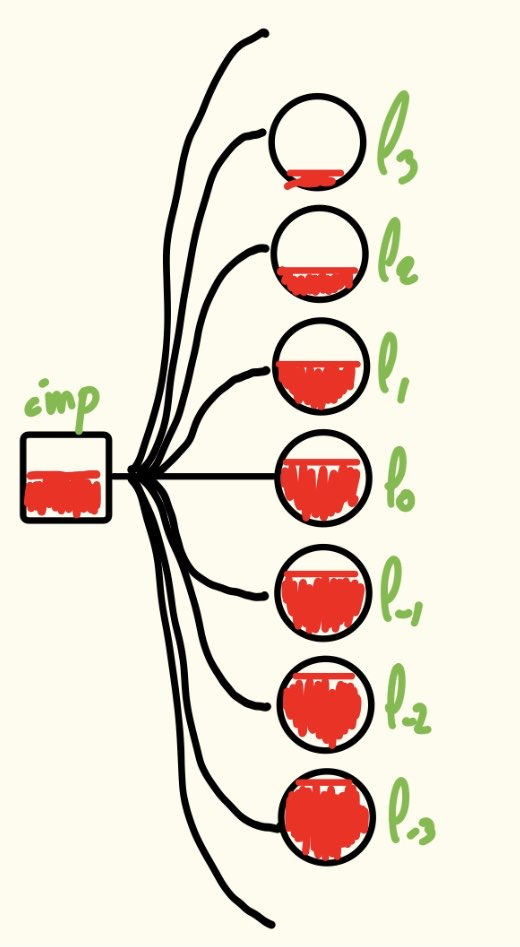
\includegraphics[width=\textwidth]{img/star_rep.jpg}
         \caption{}
         \label{subfig:star_rep}
     \end{subfigure}
    \begin{subfigure}[b]{0.27\textwidth}
         \centering
         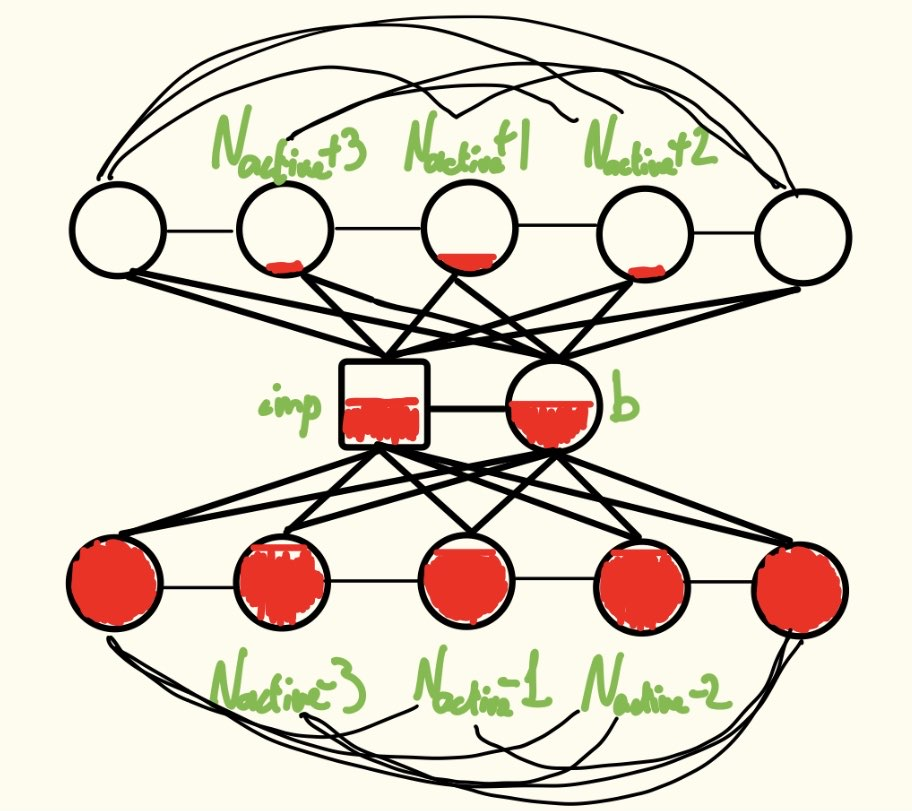
\includegraphics[width=\textwidth]{img/h_prime_rep.jpg}
         \caption{}
         \label{subfig:h_prime_rep}
     \end{subfigure}
     \begin{subfigure}[b]{0.27\textwidth}
         \centering
         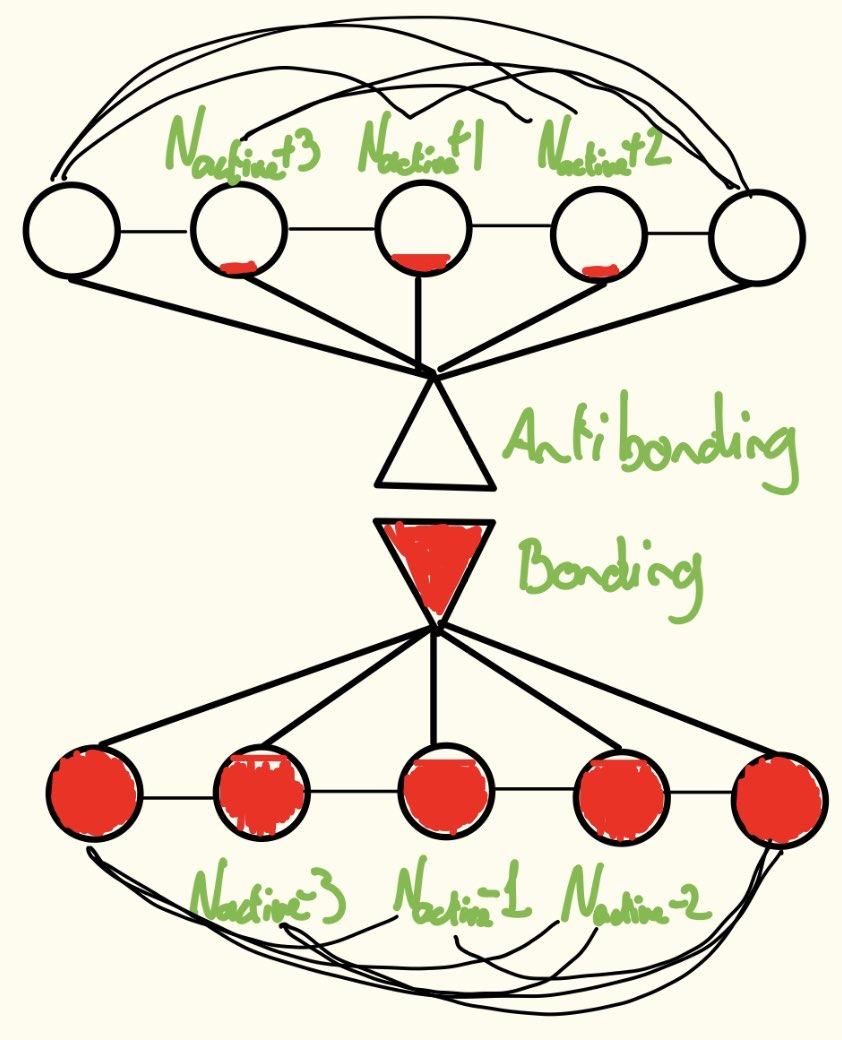
\includegraphics[width=\textwidth]{img/h_primeprime_rep.jpg}
         \caption{}
         \label{subfig:h_primeprime_rep}
     \end{subfigure}
          \begin{subfigure}[b]{0.27\textwidth}
         \centering
         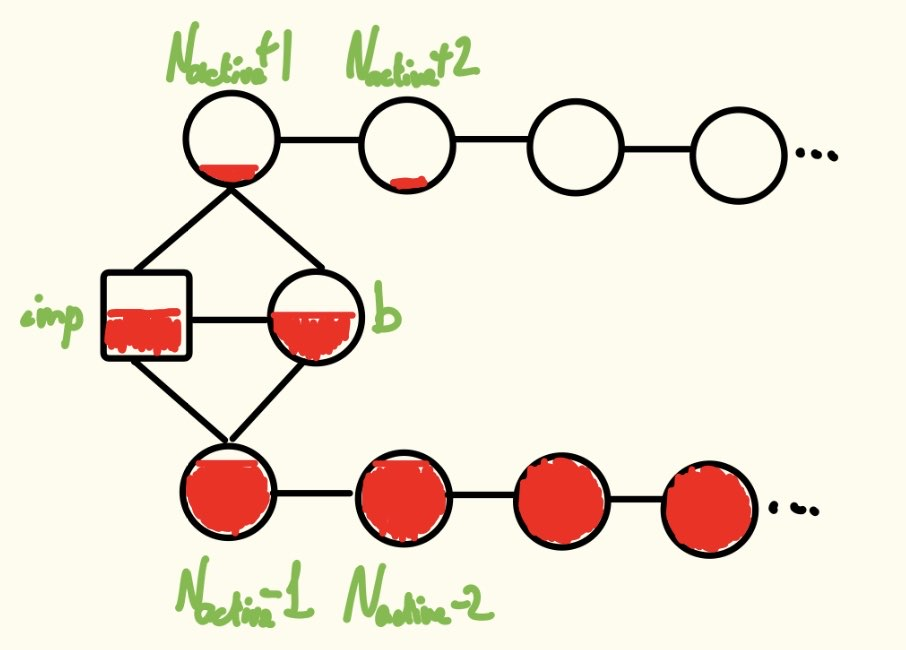
\includegraphics[width=\textwidth]{img/no_rep.jpg}
         \caption{}
         \label{subfig:no_rep}
     \end{subfigure}
     \caption{(a) Star representation of the AIM. (b) First rotation of $\hamiltonian_\star$ consisting of diagonalizing the bath density matrix. (c) Rotation of the impurity and active states to bonding and anti-bonding states with occupation of $1$ and $0$ respectively. (d) Hamiltonian in natural orbital basis after a tridiagonalization of the empty and filled parts and a rotation back to impurity and active states.}
     \label{fig:rotations}
\end{figure}
Last step corresponds to tridiagonalize each block using Lanczos or Householder transformation, and then undo the transform $C$ to recover the active and impurity site (keep locality !) (Fig. \ref{subfig:no_rep})
\begin{equation}
\hamiltonian_{NO}^{1B} = CQ^\dagger C^\dagger P^\dagger \hamiltonian_\star^{1B}PCQC^\dagger\; ;\quad
Q = 
\begin{pmatrix}
	Q_\empti & 0 \\
	0 & Q_\filled
\end{pmatrix}
\end{equation}
Therefore, the natural orbital transformation constructs two chains, one corresponding to the (almost) empty states and the other to the (almost) filled states. The impurity and active sites, which remain coupled to each other, are "located" next to the first site of each chain and are connected by a hopping term (Fig. \ref{subfig:no_rep}). The full natural-orbital Hamiltonian takes the form
\begin{align*}
\hamiltonian_{NO} & = U \occupation{0\uparrow}\occupation{0\downarrow} + \epsilon_0 (\occupation{0\uparrow} + \occupation{0\downarrow}) + \sum_\sigma \left(V_{0N_\activ-1}\creation{0\sigma}\annihilation{N_\activ-1\sigma} + V_{0N_\activ+1}\creation{0\sigma}\annihilation{N_\activ+1\sigma}\right)\\
& \quad + \epsilon_b (\occupation{b\uparrow} + \occupation{b\downarrow}) + \sum_\sigma \left(V_{bN_\activ-1}\creation{b\sigma}\annihilation{N_\activ-1\sigma} + V_{bN_\activ+1}\creation{b\sigma}\annihilation{N_\activ+1\sigma}\right) + \sum_\sigma V_{0b}\creation{b\sigma}\annihilation{0\sigma}\\
& \quad + \!\!\!\!\!
\sum_{m=1,\sigma}^{N_\activ-1}\left( \epsilon_m \occupation{m\sigma} + t_{mm+1} \creation{m\sigma}\annihilation{m+1\sigma}\right) + \!\!\!\!\!\!\!\!\!\!\sum_{n=N_\activ+1,\sigma}^{N_\bath}
\!\!\!\!\!\!\!\!\!\!
\left( \epsilon_m \occupation{m\sigma} + t_{mm+1} \creation{m\sigma}\annihilation{m+1\sigma}\right)
\end{align*}
For clarity, the complex conjugate of each off-diagonal term is not explicitly written. For the second line, the sum over the spin corresponds to the hopping between the impurity and the first site of the empty chain, with index $N_\activ-1$ (resp. the first site of the filled chain, with index $N_\activ+1$). For the third line, the first term corresponds to the on-site energy of the active site $b$. The second term describes the hopping between the empty and filled chains, while the last term corresponds to the hopping between the active site and the impurity. Finally, for the last line, the first term corresponds to the on-site energies of the filled chain and to the hopping between nearest-neighbor sites. The same applies to the second term for the empty chain. We can therefore rewrite the one-body matrix in a more compact form:
\begin{equation*}
\hamiltonian_{NO}^{1B} =
\begin{pmatrix}
 \epsilon_0 & & & V_{0N_\activ-1} & V_{0b} & V_{0N_\activ+1} & &\\
  & \epsilon_1 & t_{12} & & & & &\\
  & t_{12} & \ddots & \ddots & & & &\\
 V_{0N_\activ-1} & & \ddots & \epsilon_{N_\activ-1}  & V_{N_\activ-1b} & & &\\
  V_{0b}& & &V_{N_\activ-1b} & \epsilon_{b} & V_{N_\activ+1b}& &\\
 V_{0N_\activ+1} & & & & V_{N_\activ+1b}& \epsilon_{N_\activ+1}& \ddots & &\\
  & & & & & \ddots & \ddots &t_{N_\bath-1,N_\bath}\\
  & & & & & & t_{N_\bath-1,N_\bath} &\epsilon_{N_\bath}
\end{pmatrix}
\end{equation*}
The computational complexity still grows exponentially with the number of bath sites. As discussed above, by introducing a threshold $\epsilon$, we can truncate the trivial parts of the transformed Hamiltonian. These parts correspond to the operator $\hamiltonian_v$ in Fig. \ref{fig:no_cut} for the inactive filled sites, with $L+1$ analogous to $N_\filled$, and to the operator $\hamiltonian_c$ in Fig. \ref{fig:no_cut} for the inactive empty sites, with $L+1$ analogous to $N_\empti$. Since the occupations of these orbitals are very close to $1$ or $0$, respectively, they can be accurately approximated as fully occupied or empty orbitals and therefore treated as a single Slater determinant. Truncating these inactive parts gives us access to the relevant part of the Hamiltonian, namely the active part represented by $\hamiltonian_I$ in Fig. \ref{fig:no_cut}, which contains the non-trivial many-body physics of the system. In this way, the number of bath sites that needs to be explicitly treated in the many-body calculation can be reduced to only a few sites, with the required number depending on the chosen threshold $\epsilon$ and consequently on the desired accuracy of the calculation. For example, if we have access to the ground state $\ket{\psi_{GS}^I}$ of $\hamiltonian_I$ (DMRG, ED), the total ground-state energy is given by
\begin{equation}
E_0(\epsilon) = \bra{\psi_{GS}^I} \hamiltonian_I \ket{\psi_{GS}^I} + \!\!\!
\sum_{j=N_\filled}^{N_\bath}
\!\!\!\!
\epsilon_j
\end{equation}
where the second term corresponds to the sum of the on-site energies of the filled states.
\begin{figure}[t]
	\centering
	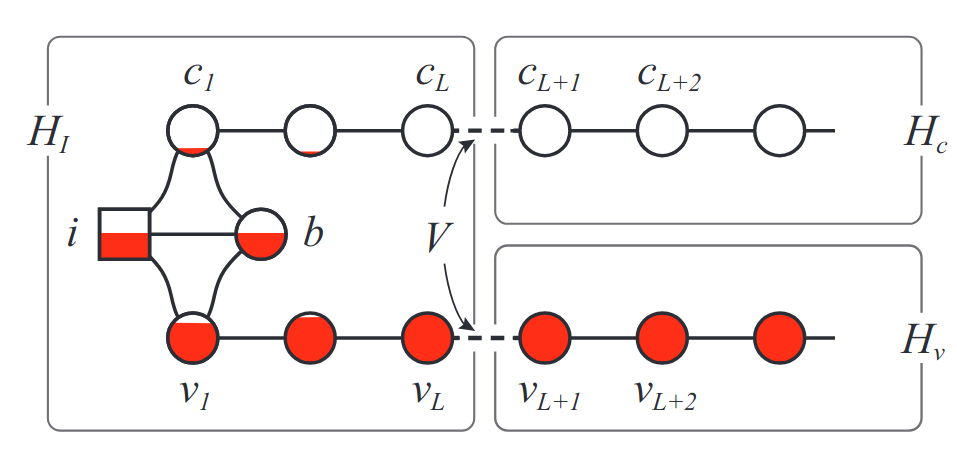
\includegraphics[width=0.45\textwidth]{img/no_rep_cut.png}
	\caption{Separating the full Anderson impurity Hamiltonian $\hamiltonian_{NO}$ defined on the natural orbitals into four parts $\hamiltonian_I$, $\hamiltonian_c$, $\hamiltonian_v$, and $V$ . Each Hamiltonian acts on the sites enclosed by its corresponding box. The hybridization operator $V$ (dashed bonds) connects $\hamiltonian_I$ to $\hamiltonian_c$ and $\hamiltonian_v$ \cite{lu_natural-orbital_2019}.}
	\label{fig:no_cut}
\end{figure}

\section{Application on an one band model}
\subsection{Discretization of the bath and groundstate calculation}
We test the natural orbital transformation on a one-band model of copper oxide $\dxy$. We first perform an \textit{ab initio} density functional theory (DFT) calculation and wannierize the $\dxy$ orbitals. We then compute the imaginary-frequency hybridization function within dynamical mean field theory (DMFT) using the continuous-time segmentation solver (CTSEG) of \textsc{Triqs}, and analytically continue the hybridization function to real frequencies using the maximum entropy method (MaxENT). We finally discretize the bath following \cite{de_vega_how_2015} (see Fig. \ref{subfig:disc_bath}). Note that the $U$ parameter of the Hubbard model, with a value of $4$ eV, is chosen such that it reproduces the experimental gap of CuO, which is approximately $1-2$ eV (Fig. \ref{subfig:disc_bath}). Fig. \ref{subfig:star_rep_cuo} shows the one-body part of the AIM for 10 bath sites \eqref{eq:star_rep}, with the impurity in the middle at index $5$, the conduction bath sites between indices $0$ and $4$, and the valence states between sites $6$ and $10$. Furthermore, I set $vmin=-2$ and $vmax=2$ in the plot in order to better visualize the hybridization.\\
I calculate the ground state of the full Hamiltonian using DMRG. Interestingly, I encounter an error in the SyTen DMRG function when I use a random initial state with zero magnetization at half-filling. I therefore also consider an initial state in which the valence sites are filled, the conduction sites are empty, and the impurity spin is initialized in a superposition, such that
\begin{align*}
	\ket{\psi_{init}} = & \frac{1}{\sqrt{2}}\ket{n_6\uparrow=1, n_6\downarrow=1, \ldots, n_{10}\downarrow=1, \mathbf{imp\uparrow=1}, \mathbf{imp\downarrow=0}, n_1\uparrow=0, \ldots, n_5\downarrow=0}\\
& + \frac{1}{\sqrt{2}}\ket{n_6\uparrow=1, n_6\downarrow=1, \ldots, n_{10}\downarrow=1, \mathbf{imp\uparrow=0}, \mathbf{imp\downarrow=1}, n_1\uparrow=0, \ldots, n_5\downarrow=0}
\end{align*}
However, the ground states do not have zero magnetization: the impurity is either spin-up or spin-down. I therefore use a more ''stable'' initial state suggested by Sebastian, in which the correct symmetries (particle number and magnetization) are preserved for each Slater determinant. The drawback is that this initial state is not half-filled.
\begin{align}
	\ket{\psi_{init}} = & \frac{1}{\sqrt{2}}\ket{n_6\uparrow=1, \ldots, \mathbf{n_{10}\uparrow=1}, \mathbf{n_{10}\downarrow=0}, \mathbf{imp\uparrow=0}, \mathbf{imp\downarrow=1}, n_1\uparrow=0, \ldots}\nonumber\\
& + \frac{1}{\sqrt{2}}\ket{n_6\uparrow=1, \ldots, \mathbf{n_{10}\uparrow=0}, \mathbf{n_{10}\downarrow=1}, \mathbf{imp\uparrow=1}, \mathbf{imp\downarrow=0}, n_1\uparrow=0, \ldots} \label{eq:init_state}
\end{align}

\begin{figure}[t]
	\centering
	\begin{subfigure}[b]{0.38\textwidth}
	\centering
	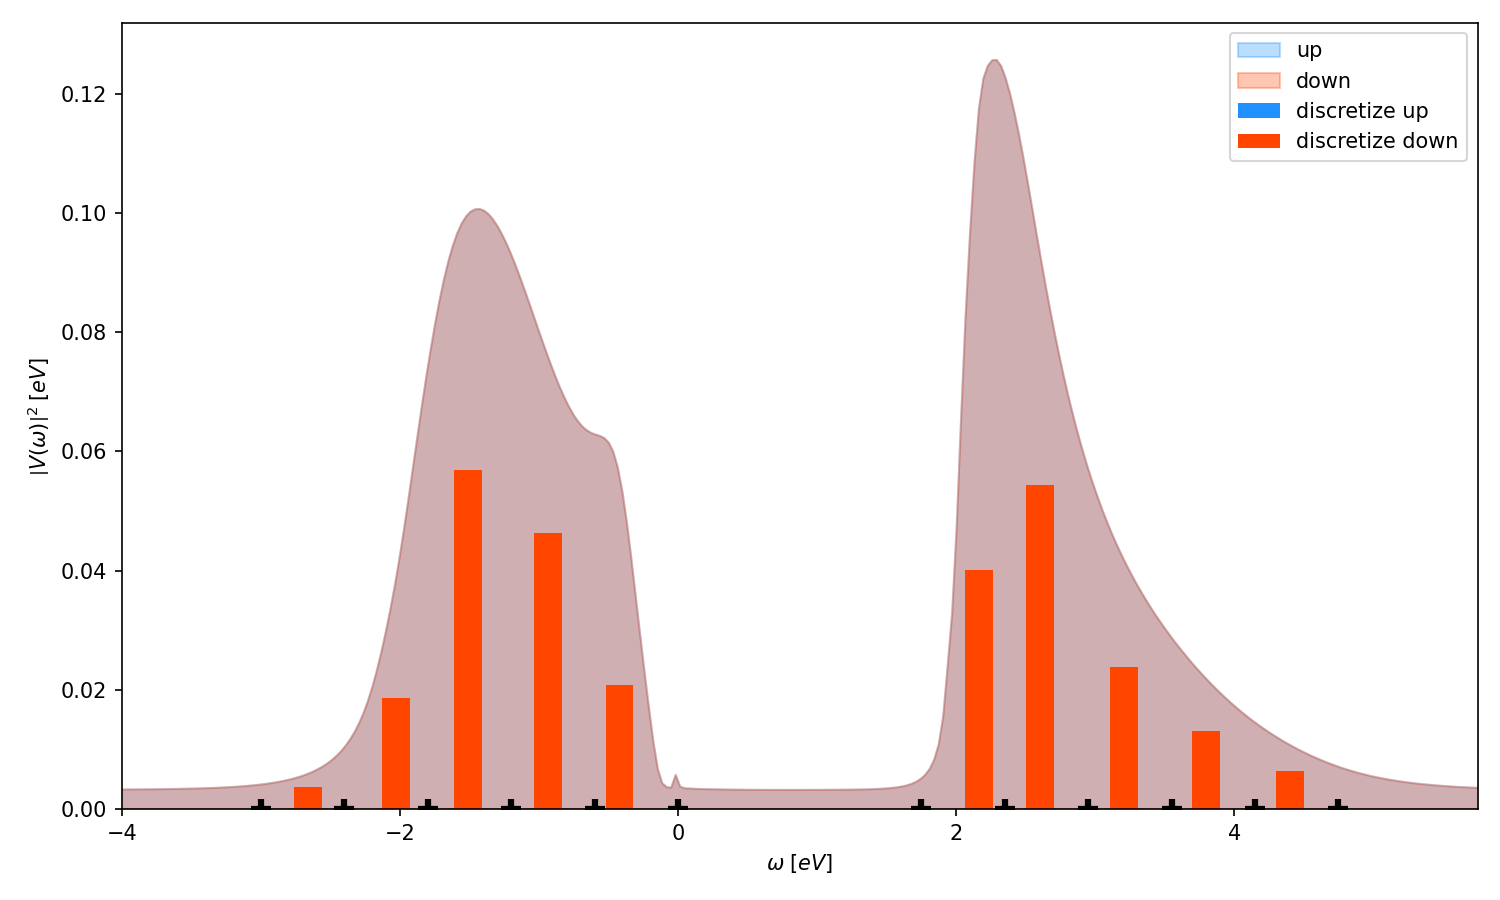
\includegraphics[width=\textwidth]{img/discr_bath_N10.png}
	\caption{}
	\label{subfig:disc_bath}
	\end{subfigure}
	\begin{subfigure}[b]{0.29\textwidth}
	\centering
	
\includegraphics[width=\textwidth]{img/star_rep_N10.png}
	\caption{}
	\label{subfig:star_rep_cuo}
	\end{subfigure}
	\begin{subfigure}[b]{0.29\textwidth}
	\centering
	
\includegraphics[width=\textwidth]{img/density_matrix_N10.png}
	\caption{}
	\label{subfig:dm_N10}
	\end{subfigure}
	\caption{(a) Filled curve: continuous bath function in real frequency. Bars: discretization of the bath using 10 bath sites. (b) One-body part of the AIM for 10 bath sites (spin-independent) \eqref{eq:star_rep}, with the impurity at the center (index $5$), the conduction bath sites at indices $0$ to $4$, and the valence states at indices $6$ to $10$. The plot is shown with $vmin=-2$ and $vmax=2$ to better visualize the hybridization. (c) Density matrix $C_{ij\sigma}$ \eqref{eq:dm} of the ground state calculated using DMRG with the initial state \eqref{eq:init_state}. Each site is represented by a $2\times2$ spin matrix.}
	\label{fig:hyb}
\end{figure}
We show in Fig. \ref{subfig:dm_N10} the density matrix $C_{ij\sigma}$ \eqref{eq:dm} of the ground state. Each site is represented by a $2\times2$ spin matrix. We first note that our system is indeed spin-independent, as expected since there is no spin interaction. Furthermore, the relevant symmetries are respected, with the correct total occupation and magnetization. Interestingly, the last valence site, site $4$, has a slightly larger occupation ($\sim 1.1$) than the impurity ($\sim 0.9$), while both have zero magnetization. We can also observe non-zero off-diagonal terms involving the impurity and the last valence site, indicating that the system is non-trivial (good for our tests!).

\subsection{Natural Orbital Transformation}
We first need to diagonalize the bath density matrix. In Fig. \ref{subfig:diagonalize_bath}, we show how close the occupations of the different bath orbitals are to $0$ or $1$. We compare, in blue, the diagonal elements of the correlation matrix with the impurity located at index $5$, and, in orange, the eigenvalues of the bath density matrix $\rho_\bath$. Note that the diagonalization mixes the bath states, so the site indices are no longer the same in the two representations. Moreover, the impurity site is not included in the bath space.\\
As mentioned in the first chapter, some of the occupations are very close to $0$ or $1$ and can therefore be considered inactive. In our case, we choose a threshold of $\epsilon=10^{-6}$, meaning that the first four bath sites are considered empty ($N_\empti = 4)$ and the last three are considered filled ($N_\filled = 8$). The active space then consists of only three bath sites, with indices $5$, $6$, and $7$. Furthermore, following the rule that the active site $b$ must have an occupation $\nu_\activ$ equal to $1-\nu_\imp$, we can identify the state with index $6$ as our active site, with an error of approximately $1 - \nu_\activ - \nu_\imp \sim 10^{-3}$.\\
In Fig. \ref{subfig:h_prime_cuo}, we present the first rotation $P$ defined by the eigenvectors of the bath density matrix \eqref{eq:bath_rotation} and applied to the hamiltonian. We place the impurity at index $0$ to follow the convention introduced in the theoretical description. However, at the end of the natural orbital transformation, it may be preferable to place the impurity next to the active site in order to reduce entanglement at the MPS level. As expected from the theory, we obtain two blocks with all-to-all hoppings: the first corresponds to the (almost) empty space $\mathcal{E}$, with indices $m\in\{1, \ldots, 5\}$, while the second corresponds to the (almost) filled space $\mathcal{F}$, with indices $n\in\{6,\ldots, 10\}$. We can also observe a strong hybridization between the impurity and the active site, as well as between the impurity and the nearest neighbors of the active site.\\
In Fig. \ref{subfig:h_prime_prime_cuo}, we show the second rotation $C$ bonding/antibonding \ref{eq:bab_rotation} applied on the hamiltonian $\hamiltonian'$. Strangely, the matrix is not well separated in two blocks (should be at site $6$) with some hybridization between the bonding and anti-bonding sites. Furthermore, when I compute the density matrix of these states, I obtain
\begin{equation}
	\rho_{AB/B} =
	\begin{pmatrix}
	\bra{AB} C \ket{AB} & \bra{B} C \ket{AB} \\
	\bra{AB} C \ket{A} & \bra{B} C \ket{B}
	\end{pmatrix}
	=
	\begin{pmatrix}
	0.243 & -0.043 \\
	-0.043 & 0.757
	\end{pmatrix}
\end{equation}
so value different of $0$ and $1$ for the occupation of the antibonding and bonding sites. Two come to my mind : either the $C$ rotation is not the correct one
\begin{figure}[t]
	\centering
	\begin{subfigure}[b]{0.31\textwidth}
	\centering
	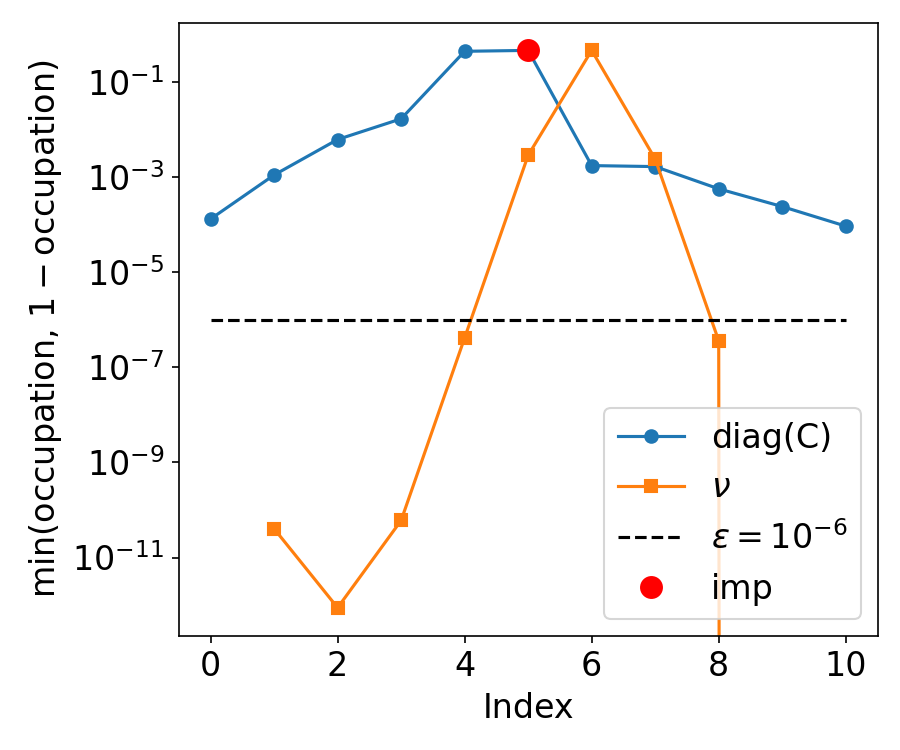
\includegraphics[width=\textwidth]{img/occupation_N10.png}
	\caption{}
	\label{subfig:diagonalize_bath}
	\end{subfigure}
	\begin{subfigure}[b]{0.33\textwidth}
	\centering
	
\includegraphics[width=\textwidth]{img/up_H1_prime_N10.png}
	\caption{}
	\label{subfig:h_prime_cuo}
	\end{subfigure}
		\begin{subfigure}[b]{0.33\textwidth}
	\centering
	
\includegraphics[width=\textwidth]{img/up_H2_prime_prime_N10.png}
	\caption{}
	\label{subfig:h_prime_prime_cuo}
	\end{subfigure}
	\caption{(a) Occupations of the different sites, showing how close they are to being empty or fully occupied (y-log scale). In blue: diagonal elements of the correlation matrix. In orange: eigenvalues of the bath density matrix $\rho_\bath$. The threshold $\epsilon=10^{-6}$ is also indicated as an example. (b) New Hamiltonian after the first rotation $P$, defined by the eigenvectors of $\rho_\bath$, applied to the star representation of the AIM. The first site corresponds to the impurity, while the sixth site corresponds to the active site.}
	\label{fig:first_rotation}
\end{figure}

\bibliographystyle{unsrt}
\bibliography{sample_}

\end{document}
